\chapter{Experiments and Results}
\label{chap:results}

This chapter presents a comprehensive empirical evaluation designed to verify each architectural hypothesis formulated in Chapter~\ref{chap:method}, strictly following the sequence of five research questions (RQ1--RQ5) established in Table~\ref{tab:rq}. To ensure scientific transparency and rigor, the experiments progress systematically from simple baselines to the complete proposed model: (1) evaluating the prognostic contribution of longitudinal temporal sequences and multimodal data integration (RQ1--RQ2); (2) testing the advantage of pairwise bilinear interactions over standard feature concatenation (RQ3); (3) quantifying the parameter compression achieved by CP decomposition and validating the streamlined RC-Free topology against all seven pairwise interaction combinations as well as the literature reference pipeline (RQ4--RQ5); and (4) verifying the practical survival stratification capability of RC-Free via time-dependent IPCW-AUC and Kaplan--Meier survival curves.

\section{Training Protocol and Convergence Dynamics}
\label{sec:experimental-protocol}
All experiments in this thesis utilize the fixed participant-level dataset partition detailed in Section~\ref{sec:data-split} (comprising 251 training, 54 validation, and 54 post-hoc test participants, corresponding to 74, 16, and 16 progression events, respectively), with all preprocessing parameters fitted exclusively on the training set. The validation set contains 480 comparable patient pairs and the post-hoc test set contains 528 comparable pairs. The initial exploratory input ablations (RQ1--RQ2) are conducted using a single random initialization; all core architectural comparisons and survival evaluations are repeated across three independent random seeds (20260727, 20260728, and 20260729), with metrics reported as sample mean $\pm$ standard deviation (SD).

Because 3D volumetric MRI sequences consume substantial GPU memory whereas the Cox partial log-likelihood objective is sensitive to small batch sizes, the training protocol is carefully configured as follows:
\begin{enumerate}
\item \emph{Optimization algorithm}: The model is optimized using AdamW \cite{loshchilov2019adamw} with an initial learning rate of $10^{-4}$, weight decay of $10^{-4}$, momentum parameters $(\beta_1,\beta_2)=(0.9,0.999)$, and gradient norm clipping at a threshold of $1.0$ \cite{pascanu2013difficulty} to ensure training stability.
\item \emph{Batch size, gradient accumulation, and mixed precision}: The physical mini-batch size is set to 6 participants combined with gradient accumulation over 2 steps prior to each weight update (with Cox risk sets computed within each individual mini-batch). Training employs FP16 mixed precision \cite{micikevicius2018mixed} to reduce memory footprint, while the log-sum-exp operations inside the Cox loss are explicitly cast to FP32 to guarantee numerical precision.
\item \emph{Valid Cox batch sampler}: A specialized batch sampler ensures that every training participant appears exactly once per epoch (42 batches per epoch) while guaranteeing that every mini-batch contains at least one valid comparable event pair. Consequently, across all three random initializations, all 4032 training mini-batch updates are strictly valid.
\item \emph{Learning rate scheduling and checkpoint selection}: Models are trained for a maximum of 100 epochs using a \texttt{ReduceLROnPlateau} scheduler \cite{pytorchReduceLROnPlateau} monitoring the validation Cox loss (halving the learning rate after 5 epochs without improvement, down to a floor of $10^{-6}$). Following an initial 10-epoch warm-up period, early stopping monitors the validation C-index (requiring a minimum improvement of 0.002 with a patience of 20 epochs); the saved model checkpoint is the one achieving the highest validation C-index.
\end{enumerate}

\begin{figure}[H]
\centering
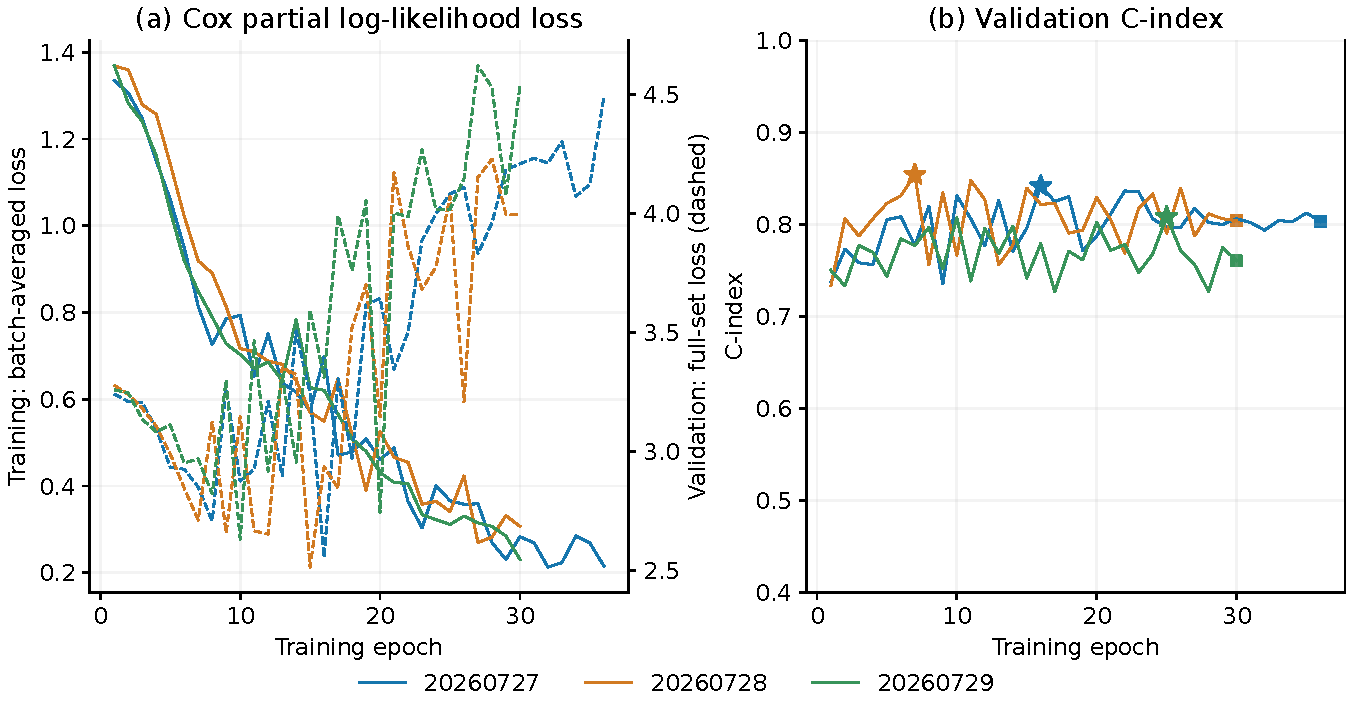
\includegraphics[width=\textwidth]{image_en/empirical-training.pdf}
\caption{Training convergence dynamics of RC-Free across three seeds}
\label{fig:empirical-training}
\captionsetup{justification=raggedright}
\caption*{Panel (a): batch-averaged training Cox loss (solid curves, left axis) and full-set validation Cox loss (dashed curves, right axis). Panel (b): validation C-index across epochs; star markers denote selected best checkpoints, and square markers denote early-stopping epochs.}
\end{figure}

The training trajectories in Figure~\ref{fig:empirical-training} demonstrate that across all three runs, the training loss decreases smoothly (from 1.33--1.37 down to 0.22--0.31), whereas the validation loss exhibits a gradual upward trend after the early epochs (from 3.24--3.28 to 3.99--4.53)---a classic signature of overfitting when optimizing deep neural networks on a modest clinical cohort. It is important to emphasize that the absolute magnitudes of the two loss axes should not be compared directly, because the Cox partial log-likelihood scales with the size of the risk set \cite{kvamme2019time} (at most 6 participants per training mini-batch versus all 54 participants on the full validation set). Because the primary objective of the task is risk ranking, I select the optimal checkpoint based on the peak validation C-index (Panel b): the three runs select checkpoints at epochs 16, 7, and 25 (achieving validation C-indices of 0.8417, 0.8542, and 0.8083, respectively) and trigger early stopping at epochs 36, 30, and 30.

\section{Longitudinal and Multimodal Ablation (RQ1--RQ2)}
First, to establish a solid empirical foundation, I conduct an exploratory ablation study addressing the first two research questions: whether longitudinal information from repeated MRI scans and the addition of radiomics and clinical scores genuinely improve risk-ranking concordance. Table~\ref{tab:exploratory} summarizes the validation C-index across progressively enriched input configurations (evaluated on seed 20260727).

\begin{table}[H]
\centering\small
\caption{Validation C-index across input configurations (seed 20260727).}
\label{tab:exploratory}
\begin{tabularx}{\linewidth}{@{}Y r@{}}
\toprule
\textbf{Model Configuration} & \textbf{C-index $\uparrow$} \\
\midrule
Last-MRI (single-timepoint baseline) & 0.7333 \\
Longitudinal MRI + T-LSTM & 0.7333 \\
Longitudinal MRI + T-LSTM + Attention & 0.7833 \\
Three-Modality Concatenation (MRI + Radiomics + Clinical) & \textbf{0.8125} \\
\bottomrule
\end{tabularx}
\end{table}

The empirical results reveal two distinct performance leaps. First, relying solely on the final hidden state of the T-LSTM over three MRI scans fails to outperform the single-timepoint Last-MRI baseline (both achieving 0.7333); however, once the additive attention mechanism is incorporated to aggregate all three visits with learned weights, the validation C-index jumps from 0.7333 to 0.7833 (+0.0500). This finding confirms that the prognostic value of longitudinal imaging is unlocked only when the model can adaptively balance contributions across visits rather than passively depending on the final recurrent state. Second, incorporating whole-brain radiomics and clinical assessment scores via simple feature concatenation further elevates the C-index to \textbf{0.8125} (+0.0292 over the best MRI-only configuration). Building upon this clear empirical evidence, all subsequent architectural experiments retain all three input modalities together with the T-LSTM and additive attention backbone.

\section{Concatenation vs. Outer-Product (RQ3)}
\label{sec:matched-fusion}
Having confirmed the indispensable contribution of all three longitudinal modalities, I next investigate the third research question (RQ3): whether explicitly modeling bilinear pairwise interactions via the outer product outperforms traditional feature concatenation. To strictly isolate the pure effect of the fusion mechanism, I hold all other architectural components fixed (including the 3D ResNet-18 backbone, 128-dimensional T-LSTM, additive attention, Breslow Cox objective, and all training hyperparameters) and ensure \emph{identical initial weights} for all shared modules across each random seed (Table~\ref{tab:matched-fusion}).

\begin{table}[H]
\centering\small
\caption{Validation C-index of Concatenation vs. Full Outer-Product (mean $\pm$ SD).}
\label{tab:matched-fusion}
\begin{tabularx}{\linewidth}{@{}Y r@{}}
\toprule
\textbf{Fusion Architecture} & \textbf{C-index $\uparrow$} \\
\midrule
Concatenation & $0.8149\pm0.0214$ \\
Full Outer-Product & $\mathbf{0.8285\pm0.0272}$ \\
\bottomrule
\end{tabularx}
\end{table}

Under strictly matched initialization conditions, the Full Outer-Product variant achieves a mean validation C-index of \textbf{0.8285}, outperforming the 0.8149 achieved by standard feature concatenation (a mean gain of \textbf{0.0135} computed on unrounded values). This consistent improvement demonstrates that explicitly constructing second-order cross-products enables the neural network to exploit inter-modality relationships more effectively. This finding establishes Full Outer-Product as the reference starting point for two subsequent architectural refinements: compressing interaction parameters via CP decomposition and pruning redundant pairwise interactions.

\section{CP Compression and Topology Search (RQ4--RQ5)}
\label{sec:cp-results}
\label{sec:ablation-results}
\label{sec:rcfree-multiseed}
\label{sec:standardized-benchmark}
\label{sec:paper-adaptation-results}

Starting from the Full Outer-Product architecture, I perform two controlled simplification steps across the same three random seeds (20260727--20260729), and subsequently benchmark the resulting architecture against the adapted CNN--PCA--T-LSTM reference pipeline to address RQ4 and RQ5.

\subsection{Parameter Reduction via CP Decomposition (RQ4)}
\label{sec:computational-efficiency}
When transitioning from Full Outer-Product to Full CP, all modality encoders, gated residual routing branches, and downstream temporal modules remain completely unchanged; the sole modification is that the initial bilinear layer of the three pairs (MR, MC, and RC) is parameterized via CP decomposition with ranks 8, 8, and 4, respectively (Table~\ref{tab:cpconfig}). Table~\ref{tab:interaction-parameters} compares the resulting parameter counts across three distinct architectural scopes.

\begin{table}[H]
\centering\small
\caption{Parameter counts of Full Outer-Product and Full CP across scopes.}
\label{tab:interaction-parameters}
\begin{tabularx}{\linewidth}{@{}Y r r@{}}
\toprule
\textbf{Architectural Scope} & \textbf{Full Outer-Product} & \textbf{Full CP} \\
\midrule
Three initial bilinear layers & 229696 & \textbf{3712} \\
Three complete interaction blocks (including MLPs) & 248608 & \textbf{22624} \\
Entire network & 33760941 & \textbf{33534957} \\
\bottomrule
\end{tabularx}
\end{table}

The figures in Table~\ref{tab:interaction-parameters} highlight the dramatic local compression achieved by CP decomposition: across the three initial bilinear layers, the number of learnable parameters drops from 229696 down to just 3712, representing a \textbf{98.38\% reduction}; when accounting for the entire interaction blocks (including their downstream MLPs), the parameter reduction remains an impressive \textbf{90.90\%}. By contrast, at the whole-network scale, the relative reduction is approximately 0.67\% because the 3D ResNet-18 backbone of the MRI branch dominates the total parameter budget and remains unchanged. In exchange for this substantial structural compression at the interaction layer, the mean validation C-index of Full CP (0.8278) trails Full Outer-Product (0.8344) by only a minor margin of 0.0066 on the main benchmark suite (Table~\ref{tab:standard-bench}). Rather than stopping at Full CP, the next step examines whether pruning redundant pairwise interactions can simultaneously save additional parameters and fully recover ranking concordance.

\subsection{Seven-Topology Benchmark and RC-Free (RQ5)}
\label{sec:new-topology}
To test the hypothesis that retaining all three pairwise interactions is unnecessary, I systematically evaluate all seven CP topologies containing at least one active interaction pair (comprising three single-pair variants, three two-pair variants, and the three-pair Full CP model). Crucially, \emph{every topology retains all three input modalities and their direct representation pathways}; the only difference lies in which pairwise bilinear interactions are activated. Table~\ref{tab:new-topology} reports the empirical results across the three random initializations.

\begin{table}[H]
\centering\small
\caption{Parameters and validation C-index across seven CP topologies (mean $\pm$ SD).}
\label{tab:new-topology}
\begin{tabularx}{\linewidth}{@{}Y c r r@{}}
\toprule
\textbf{Topology} & \textbf{Pairs / routes} & \textbf{Parameters} & \textbf{C-index $\uparrow$} \\
\midrule
MR-only & 1 / 2 & 33484165 & $0.8299\pm0.0267$ \\
MC-only & 1 / 2 & 33484037 & $0.8236\pm0.0237$ \\
RC-only & 1 / 2 & 33464165 & $0.8319\pm0.0214$ \\
RC-Free (MR+MC) & 2 / 4 & 33519497 & $\mathbf{0.8347\pm0.0237}$ \\
MR-Free (MC+RC) & 2 / 4 & 33499625 & $0.8243\pm0.0249$ \\
MC-Free (MR+RC) & 2 / 4 & 33499753 & $0.8222\pm0.0156$ \\
Full CP & 3 / 6 & 33534957 & $0.8278\pm0.0250$ \\
\bottomrule
\end{tabularx}
\end{table}

Across all seven surveyed topologies, \textbf{RC-Free (MR+MC)} achieves the highest mean validation C-index (\textbf{0.8347}), followed by the single-pair RC-only configuration (0.8319). Notably, compared with Full CP, omitting the direct RC interaction reduces the number of gated residual branches from six to four, \textbf{saves 15460 parameters}, and elevates the mean validation C-index from 0.8278 to 0.8347. Considering domain-grounded architectural design (positioning MRI as the central hub), ranking accuracy, and parameter compactness together, RC-Free emerges as the optimal architecture for in-depth survival stratification analysis.

\subsection{Overall Comparison Against the Reference Pipeline}
Table~\ref{tab:standard-bench} benchmarks the proposed RC-Free model against Full Outer-Product, Full CP, and the adapted re-implementation of the CNN--PCA--T-LSTM pipeline of Aghajanian et al. on the same validation set.

\begin{table}[H]
\centering\small
\caption{Validation C-index across benchmark models (mean $\pm$ SD).}
\label{tab:standard-bench}
\begin{tabularx}{\linewidth}{@{}Y r r c@{}}
\toprule
\textbf{Model} & \textbf{C-index $\uparrow$} & \textbf{Parameters} & \textbf{Pairs / routes} \\
\midrule
CNN--PCA--T-LSTM & $0.7417\pm0.0693$ & $33213122$ & 0 / 0 \\
Full Outer-Product & $0.8344\pm0.0148$ & $33760941$ & 3 / 6 \\
Full CP Pairwise & $0.8278\pm0.0250$ & $33534957$ & 3 / 6 \\
RC-Free Pairwise & $\mathbf{0.8347\pm0.0237}$ & $33519497$ & 2 / 4 \\
\bottomrule
\end{tabularx}
\caption*{\textit{Note.} All figures in this table are evaluated on the same validation set. The reference CNN--PCA--T-LSTM model follows the pipeline of Aghajanian et al.~\cite{aghajanian2025longitudinal} with the adaptations summarized in Table~\ref{tab:reference-methods}.}
\end{table}


Compared with Full Outer-Product, the RC-Free architecture \textbf{reduces 241444 parameters} (streamlining from 3 pairs / 6 routes down to 2 pairs / 4 routes) while achieving the highest mean validation C-index (\textbf{0.8347} versus 0.8344). More importantly, when benchmarked against the CNN--PCA--T-LSTM reference pipeline ($0.7417\pm0.0693$), all three end-to-end multimodal fusion architectures outperform the reference baseline by approximately 0.086 to 0.093 C-index points, while reducing cross-seed standard deviation by nearly threefold (0.0148--0.0250 versus 0.0693). This result demonstrates that end-to-end training combining a pretrained 3D volumetric encoder with explicit cross-modal interactions delivers superior ranking concordance and numerical stability compared with a decoupled two-stage pipeline relying solely on PCA-compressed imaging features.

\section{Survival Analysis of the RC-Free Model}
\label{sec:posthoc-test}
\label{sec:survival-results}
With the optimal RC-Free architecture selected, this section conducts an in-depth evaluation of the estimated log-risk scores $\eta_i$ across both the validation set (primary evaluation) and the held-out post-hoc test set from two complementary perspectives: horizon-specific discrimination (IPCW-AUC) and longitudinal risk-group stratification (Kaplan--Meier curves).

\subsection{C-index and Time-Dependent AUC at 2, 3, and 5 Years}
Table~\ref{tab:survival-metrics} summarizes the global C-index alongside the time-dependent IPCW-AUC values at three clinical horizons, accompanied by Table~\ref{tab:horizon-support} reporting the exact counts of cumulative cases, dynamic controls, and right-censored subjects at each horizon to clarify the sample support underlying each estimate.

\begin{table}[H]
\centering\small
\caption{C-index and IPCW time-dependent AUC of RC-Free (mean $\pm$ SD).}
\label{tab:survival-metrics}
\begin{tabularx}{\linewidth}{@{}Y r r@{}}
\toprule
\textbf{Metric} & \textbf{Validation (primary)} & \textbf{Test (post-hoc)} \\
\midrule
C-index & $\mathbf{0.8347\pm0.0237}$ & $\mathbf{0.8466\pm0.0267}$ \\
2-year AUC & $\mathbf{0.9805\pm0.0149}$ & $0.8858\pm0.0245$ \\
3-year AUC & $\mathbf{0.9788\pm0.0162}$ & $0.8770\pm0.0318$ \\
5-year AUC & $0.7889\pm0.0632$ & $0.8483\pm0.0508$ \\
\bottomrule
\end{tabularx}
\caption*{\textit{Note.} Each evaluation split comprises 54 participants with 16 observed events across three random initializations.}
\end{table}

\begin{table}[H]
\centering\small
\caption[Participant counts by outcome status and uncensored survival probability at each horizon]{At each horizon, the three counts denote cumulative cases up to the horizon, dynamic controls remaining under follow-up beyond the horizon, and subjects right-censored at or before the horizon, respectively. The uncensored probability $\widehat G(h)$ is estimated from the training set.}
\label{tab:horizon-support}
\begin{tabularx}{\linewidth}{@{}c Y Y r@{}}
\toprule
\textbf{Horizon (years)} & \textbf{Validation} & \textbf{Test (post-hoc)} & \textbf{$\widehat G(h)$} \\
\midrule
2 & 7 / 37 / 10 & 8 / 37 / 9 & $0.831$ \\
3 & 7 / 34 / 13 & 11 / 29 / 14 & $0.697$ \\
5 & 12 / 19 / 23 & 14 / 16 / 24 & $0.475$ \\
\bottomrule
\end{tabularx}
\end{table}


On the validation set, RC-Free achieves strong discrimination at the earlier horizons, recording an AUC of \textbf{0.9805} at 2 years and \textbf{0.9788} at 3 years, before decreasing to 0.7889 at the 5-year horizon. Cross-referencing with the sample support in Table~\ref{tab:horizon-support} reveals that this trajectory directly reflects the underlying sample structure at each time point. At the 2- and 3-year horizons, the validation set contains only \textbf{7 cumulative cases}, meaning that finite-sample variability is naturally non-negligible. By the 5-year horizon, although the number of cumulative cases increases to 12, the number of dynamic controls remaining under active follow-up beyond 5 years drops sharply from 37 down to 19 due to 23 subjects being right-censored earlier. Figure~\ref{fig:empirical-roc} visually reflects this phenomenon: at the 5-year validation horizon, the ROC curves across the three seeds exhibit wider dispersion (SD increasing to 0.0632) compared with the tight clustering at the 2- and 3-year horizons. Reassuringly, on the independent post-hoc test set, discrimination remains highly consistent across all three horizons (achieving AUCs of 0.8858, 0.8770, and 0.8483 at 2, 3, and 5 years, respectively), accompanied by an overall C-index of $0.8466\pm0.0267$.

\begin{figure}[H]
\centering
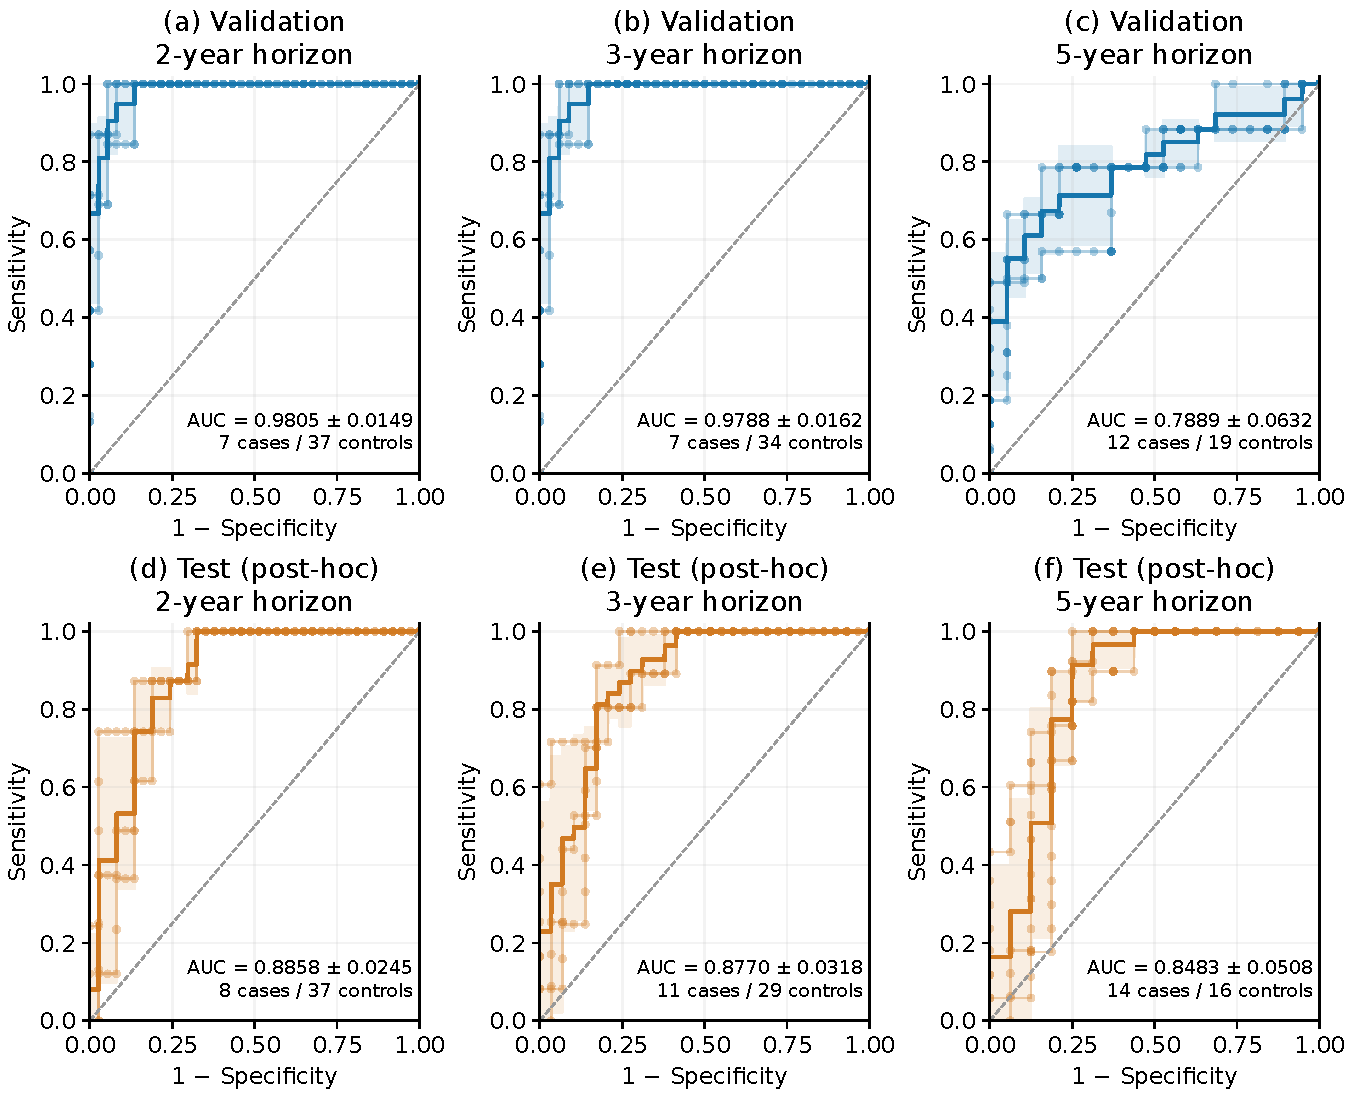
\includegraphics[width=\textwidth,trim=0bp 263.8bp 0bp 0bp,clip]{image_en/empirical-ipcw-roc.pdf}\\[3.6cm]
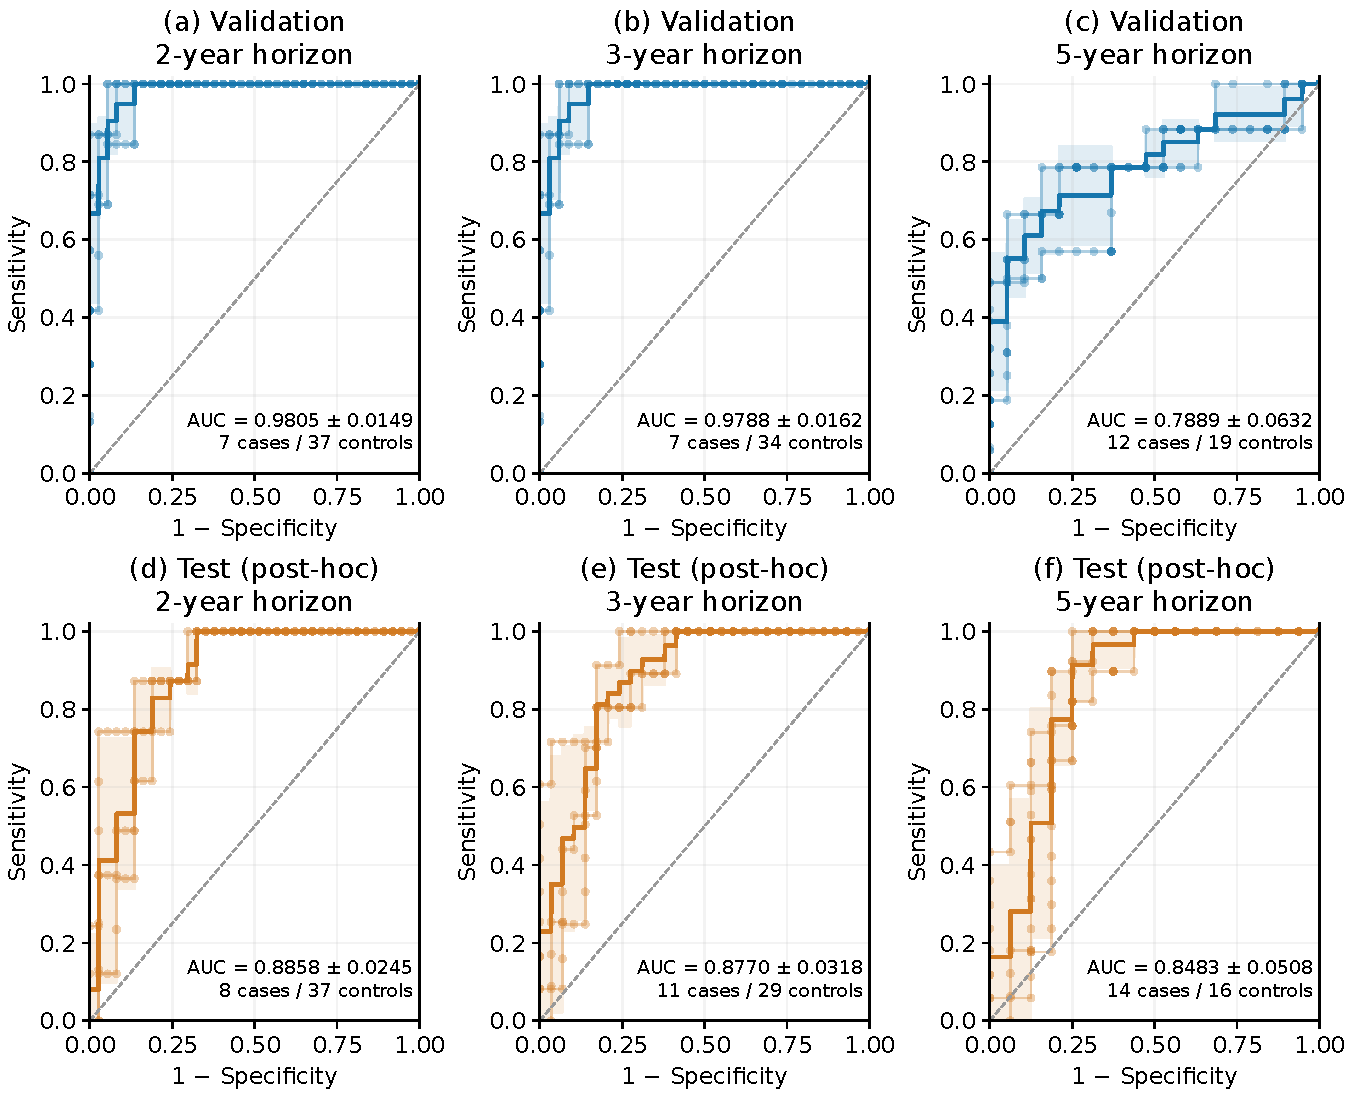
\includegraphics[width=\textwidth,trim=0bp 0bp 0bp 263.0bp,clip]{image_en/empirical-ipcw-roc.pdf}
\caption{IPCW time-dependent ROC curves of RC-Free at 2, 3, and 5 years}
\label{fig:empirical-roc}
\captionsetup{justification=raggedright}
\caption*{Top row: validation set; bottom row: post-hoc test set. Thin curves and circular markers represent individual seeds; bold curves denote the across-seed mean; shaded bands indicate $\pm1$ SD. The diagonal dashed line represents random guessing.}
\end{figure}

\clearpage
\subsection{Kaplan--Meier Stratification via Consensus Risk Groups}
Figure~\ref{fig:survival-km} and Table~\ref{tab:km-statistics} evaluate the model's ability to stratify participants into high- and low-risk progression groups (defined using the fixed training-set median risk cutoff and majority-vote consensus across the three random initializations).

\begin{figure}[H]
\centering
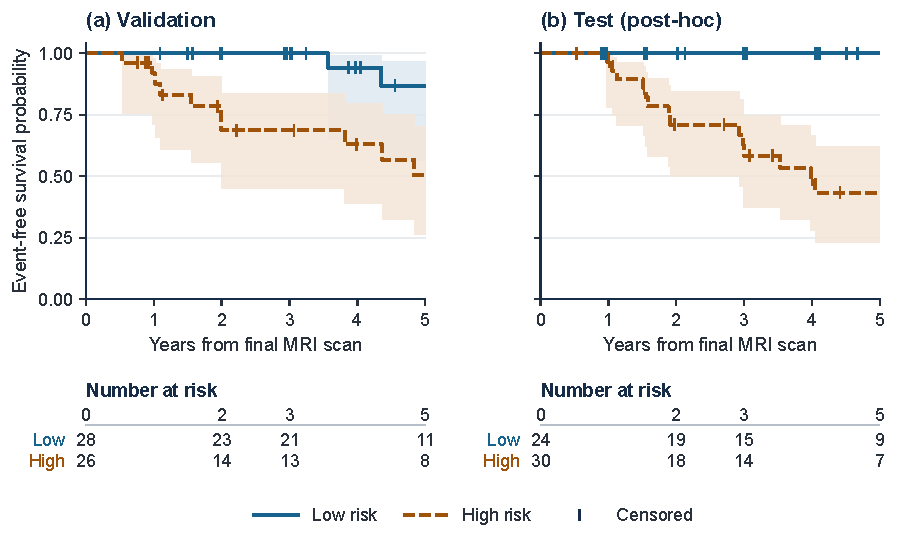
\includegraphics[width=\textwidth]{image_en/survival-km.pdf}
\caption{Kaplan--Meier survival curves across RC-Free risk groups}
\label{fig:survival-km}
\captionsetup{justification=raggedright}
\caption*{Panel (a): validation set; Panel (b): post-hoc test set. Shaded bands represent 95\% confidence intervals; vertical tick marks indicate right-censoring times. The tables below the horizontal axes report the number of subjects remaining at risk at each time horizon.}
\end{figure}

\begin{table}[H]
\centering\small
\caption{Log-rank test, hazard ratio (HR), and PH assumption test.}
\label{tab:km-statistics}
\begin{tabularx}{\linewidth}{@{}Y r r r r@{}}
\toprule
\textbf{Dataset split} & \textbf{Log-rank $p$} & \textbf{HR} & \textbf{95\% CI} & \textbf{$p$ (PH)} \\
\midrule
Validation & $\mathbf{0.0134}$ & $\mathbf{3.79}$ & $1.22$--$11.78$ & $0.1031$ \\
Test (post-hoc) & $\mathbf{<0.001}$ & $\mathbf{16.17}$ & $2.12$--$123.17$ & $0.1592$ \\
\bottomrule
\end{tabularx}
\end{table}


The two survival curves separate clearly across both dataset splits, confirming the strong risk-stratification capability of the proposed model. On the validation set, the low-risk group (28 participants) records only 4 progression events, whereas the high-risk group (26 participants) experiences 12 progression events---three times as many as the low-risk group; the log-rank test confirms statistically significant separation (\textbf{$p=0.0134$}), with an estimated hazard ratio of \textbf{HR = 3.79} (95\% CI: 1.22--11.78). On the post-hoc test set, the separation is even more pronounced: among the 24 participants assigned to the low-risk group, virtually no cognitive progression occurs during the first 5 years of follow-up (with only a single event recorded after year 5), in stark contrast to 15 progression events among the 30 participants in the high-risk group, yielding \textbf{log-rank $p<0.001$} and \textbf{HR = 16.17} (95\% CI: 2.12--123.17). The wide confidence interval of the hazard ratio on the test set arises directly from the fact that the low-risk reference group contains only a single event in the denominator; even so, the lower bound of the 95\% confidence interval still reaches 2.12, confirming a substantially elevated progression rate in the high-risk group. Furthermore, the Schoenfeld residuals test yields $p=0.1031$ on the validation set and $p=0.1592$ on the test set (both exceeding 0.05), indicating no evidence against the proportional hazards assumption over time and confirming that RC-Free delivers both accurate global ranking and reliable longitudinal survival stratification.

\section{Answers to the Research Questions}
\label{sec:rq-results}
Synthesizing the empirical investigations presented throughout this chapter, the five research questions posed in Table~\ref{tab:rq} are restated and answered in detail below:

\begin{description}[leftmargin=1.35cm,labelwidth=1.1cm,itemsep=.4em]
\item[RQ1.] \emph{Do longitudinal multi-timepoint MRI scans provide superior risk discrimination compared with using only the final MRI scan?} Yes, provided that the visit sequence is aggregated via adaptive attention. Relying solely on the final T-LSTM state matches the single-scan \emph{Last-MRI} baseline (validation C-index 0.7333), whereas adding additive attention across all three irregularly spaced visits raises the C-index to \textbf{0.7833} (+0.0500, Table~\ref{tab:exploratory}), capturing within-person atrophy dynamics.
\item[RQ2.] \emph{Does incorporating radiomics and clinical scores improve risk discrimination over using MRI alone?} Yes. Adding whole-brain PyRadiomics descriptors (16 PCA components) and clinical MMSE/CDR assessments (9 scores with 9 missingness indicators) elevates the validation C-index from 0.7833 to \textbf{0.8125} (+0.0292, Table~\ref{tab:exploratory}), confirming complementary value across macroscopic anatomy, tissue texture statistics, and cognitive-functional scales.
\item[RQ3.] \emph{Is pairwise bilinear interaction more effective than simple feature concatenation?} Yes. Under matched initial weights for all shared modules across three random seeds, \emph{Full Outer-Product} fusion achieves a mean validation C-index of \textbf{0.8285} versus 0.8149 for \emph{Concatenation}---a mean gain of \textbf{0.0135} on unrounded values (Table~\ref{tab:matched-fusion})---by explicitly modeling second-order cross-modal products through gated residual routes.
\item[RQ4.] \emph{How many interaction-layer parameters does CP decomposition reduce, and how does it affect the C-index?} Low-rank CP factorization ($Q=8$ for MR and MC; $Q=4$ for RC) reduces the three initial bilinear layers by \textbf{98.38\%} (from 229696 to 3712 parameters) and the three complete interaction blocks by \textbf{90.90\%} (0.67\% whole-network reduction, Table~\ref{tab:interaction-parameters}), while incurring only a minor 0.0066 difference in mean validation C-index between \emph{Full CP} (0.8278) and \emph{Full Outer-Product} (0.8344, Table~\ref{tab:standard-bench}).
\item[RQ5.] \emph{Can redundant pairwise interactions be pruned while preserving risk discrimination performance?} Yes---pruning the direct RC pair while keeping MRI as the central hub in \textbf{RC-Free (MR+MC)} reduces gated routes from six to four, saves \textbf{15460 parameters} over \emph{Full CP} (241444 over \emph{Full Outer-Product}), and attains the highest mean validation C-index among all seven CP topologies (\textbf{0.8347}, Table~\ref{tab:new-topology}; post-hoc test \textbf{0.8466}, Table~\ref{tab:survival-metrics}), with significant Kaplan--Meier separation on validation ($p=0.0134$, $\mathrm{HR}=3.79$) and post-hoc test ($p<0.001$, $\mathrm{HR}=16.17$, Table~\ref{tab:km-statistics}).
\end{description}
